\clearpage
\chapter{Mastery Workbook 4}

% Chapter page
\section{Sets And Functions Workbook}

\horizontalline{0}{0}

\begin{center}
    \Large{\textbf{I have neither given nor received unauthorized assistance.}}
    \horizontalline{0}{0}
    \large{\textbf{Taylor James Larrechea}}
    \horizontalline{0}{0}
\end{center}

% Problem 1
\begin{problem}{Problem 1}
    \begin{statement}{Problem Statement}
        Prove the “other” DeMorgan’s law following Chris’ examples in the set video - slide 26 (similar to example 11 p. 131).
    \end{statement}

    \begin{Highlight}[Solution]
        \noindent \textbf{Theorem:} $\overline{A \cup B} = \overline{A} \cap \overline{B}$ \vspace*{1em}

        \noindent \textbf{Direct Proof:}

        \horizontalline{0}{-1.5}
        \begin{align*}
            \overline{A \cup B} & = \{x | x \notin A \cup B \} & \text{(Definition of complement)} \\
            & = \{x | \neg (x \in A \cup B) \} & \text{(Definition of not in)} \\
            & = \{x | \neg (x \in A \vee \hspace*{1pt} x \in B)\} & \text{(Definition of union)} \\
            & = \{x | \neg (x \in A) \wedge \neg (x \in B) \} & \text{(DeMorgan’s Law)} \\
            & = \{x | x \notin A \wedge x \notin B \} & \text{(Definition of not in)} \\
            & = \{x | x \in \overline{A} \wedge x \in \overline{B} \} & \text{(Definition of complement)} \\
            & = \{x | x \in \overline{A} \cap \overline{B} \} & \text{(Definition of intersection)} \\
            & = \overline{A} \cap \overline{B} & \text{(Intersection of complements)}
        \end{align*}
        \horizontalline{-1}{0}
        Consequently, we have shown that $\overline{A \cup B} = \overline{A} \cap \overline{B}$ is indeed a true statement. \qed
    \end{Highlight}
\end{problem}

% Problem 1 Summary
\begin{summary}{Problem 1 Summary}
    \begin{statement}{Procedure}
        \begin{itemize}
            \item Use the definition of set identities in tandem with logical equivalences to arrive at the theorem that is presented to us
        \end{itemize}
    \end{statement}
    \begin{statement}{Key Concepts}
        \begin{itemize}
            \item \textbf{Theorem}: The theorem in question states that the complement of the union of two sets, $\overline{A \cup B}$, is equal to the intersection of their complements, 
            $\overline{A} \cap \overline{B}$.
            \item \textbf{Direct Proof}: This is a type of proof technique used to establish the truth of a statement by providing a step-by-step logical argument
            \item \textbf{Definition of Complement}: The complement of a set $A$, denoted as $\overline{A}$, consists of all elements not in $A$
            \item \textbf{Definition of Not In}: This is a way of expressing that an element does not belong to a set, denoted as $\notin$
            \item \textbf{Definition of Union}: The union of two sets, denoted as $A \cup B$, consists of all elements that belong to either set $A$ or set $B$, or both
            \item \textbf{DeMorgan’s Law}: This is a set theory law that relates the complement of a union to the intersection of complements and vice versa
            \item \textbf{Intersection of Complements}: This is the operation of finding elements that are in both the complements of two sets
            \item \textbf{Logical Equivalence}: The proof demonstrates that $\overline{A \cup B} = \overline{A} \cap \overline{B}$ is a logically equivalent statement by showing each step of the 
            logical argument
        \end{itemize}
    \end{statement}
    \begin{statement}{Variations}
        \begin{itemize}
            \item We could be asked to prove the other De Morgans Law for sets
            \begin{itemize}
                \item In this case we would use the same properties just in a different format
            \end{itemize}
        \end{itemize}
    \end{statement}
\end{summary}

% Problem 2
\begin{problem}{Problem 2}
    \begin{statement}{Problem Statement}
        From Rosen, page 136, do \#1-4, on this page (and next if needed) explain the important ideas of these problems with examples, insights and notes.
    \end{statement}

    \begin{Highlight}[Solution - \#1]
        \noindent \textbf{Question:} Let $A$ be the set of students who live within one mile of school and let B be the set of students who walk to classes. Describe the students in each of these sets.
        
        \begin{enumerate}[label=(\alph*)]
            \item $A \cap B =$ The set of students who live within one mile of the school and walk to classes. 
            \item $A \cup B =$ The set of students who live within one mile of the school or who walk to classes.
            \item $A - B =$ The set of students who live withing one mile of the school but do not walk to classes.
            \item $B - A =$ The set of students who walk to classes but who do not live within one mile of the school.
        \end{enumerate}
    \end{Highlight}

    \begin{Highlight}[Solution - \#2]
        \noindent \textbf{Question:} Suppose that $A$ is the set of sophomores at your school and $B$ is the set of students in discrete mathematics at your school. Express each of these sets in terms 
        of $A$ and $B$.

        \begin{enumerate}[label=(\alph*)]
            \item The set of sophomores taking discrete mathematics in your school: $A \cap B$
            \item The set of sophomores at your school who are not taking discrete mathematics: $A - B$
            \item The set of students at your school who either are sophomores or are taking discrete mathematics: $A \cup B$
            \item The set of students at your school who either are not sophomores or are not taking discrete mathematics: $\overline{A} \cup \overline{B}$
        \end{enumerate}
    \end{Highlight}

    \begin{Highlight}[Solution - \#3]
        \noindent \textbf{Question:} Let $A = \{ 1, 2, 3, 4, 5\}$ and $B = \{ 0, 3, 6\}$. Find

        \begin{enumerate}[label=(\alph*)]
            \item $A \cup B = \{0,1,2,3,4,5,6\}$
            \item $A \cap B = \{3\}$
            \item $A - B = \{1,2,4,5\}$
            \item $B - A = \{0,6\}$
        \end{enumerate}
    \end{Highlight}

    \begin{Highlight}[Solution - \#4]
        \noindent \textbf{Question:} Let $A = \{ a, b, c, d, e\}$ and $B = \{ a, b, c, d, e, f, g, h\}$. Find

        \begin{enumerate}[label=(\alph*)]
            \item $A \cup B = \{a,b,c,d,e,f,g,h\}$
            \item $A \cap B = \{a,b,c,d,e\}$
            \item $A - B = \{\emptyset\}$
            \item $B - A = \{f,g,h\}$
        \end{enumerate}
    \end{Highlight}

    \begin{Highlight}[Insights]
        It appears that the union operator $\cup$ is a collection of all elements between both sets. On the contrary, the intersection operator $\cap$ is looking for elements that exist in both sets.
        Moreover, the difference between sets is looking at the what elements exist in one set and not the other. The complement of a set, such as the set $\{A\}$ acts like the negation in propositional
        logic. Overall, there are a lot of similarities between set logic and propositional logic, just with different symbols.
    \end{Highlight}
\end{problem}

% Problem 2 Summary
\begin{summary}{Problem 2 Summary}
    \begin{statement}{Procedure}
        \begin{enumerate}
            \item Problem 1
            \begin{itemize}
                \item Use the definition of union, intersection, and difference to translate the quantities from set notation to english
            \end{itemize}
            \item Problem 2
            \begin{itemize}
                \item Use the definition of union, intersection, and difference to translate the quantities from set notation to english
            \end{itemize}
            \item Problem 3
            \begin{itemize}
                \item Use the definition of union, intersection, and difference to find the values associated with the given set
            \end{itemize}
            \item Problem 4
            \begin{itemize}
                \item Use the definition of union, intersection, and difference to find the values associated with the given set
            \end{itemize}
        \end{enumerate}
    \end{statement}
    \begin{statement}{Key Concepts}
        \begin{itemize}
            \item \textbf{Sets $A$ and $B$:} These sets are defined as $A = \{1, 2, 3, 4, 5\}$ and $B = \{0, 3, 6\}$
            \item \textbf{Union ( $\cup$ ):} The union of sets $A$ and $B$, denoted as $A \cup B$, contains all unique elements that belong to either set $A$ or set $B$, or both
            \item \textbf{Intersection ( $\cap$ ):} The intersection of sets $A$ and $B$, denoted as $A \cap B$, consists of all elements that are common to both sets $A$ and $B$. In other words, it 
            contains only the elements that appear in both sets
            \item \textbf{Set Difference ( $-$ ):} The set difference between sets $A$ and $B$, denoted as $A - B$, contains all elements that belong to set $A$ but not to set $B$. It essentially 
            removes the elements of set $B$ from set $A$
            \item \textbf{Logical Notation}: In this context, logical notation such as union ($\cup$), intersection ($\cap$), and set difference ($-$) is used to manipulate and describe the relationships 
            between sets
            \item \textbf{Result}: The results of the specified operations between sets $A$ and $B$ are presented for each part (a, b, c, d) of the problem
        \end{itemize}
    \end{statement}
    \begin{statement}{Variations}
        \begin{itemize}
            \item We could be given different sets to find the union, intersection, and difference of
            \begin{itemize}
                \item We would then just use the definition of union, intersection, and difference for sets with these new sets
            \end{itemize}
        \end{itemize}
    \end{statement}
\end{summary}

% Problem 3
\begin{problem}{Problem 3}
    \begin{statement}{Problem Statement}
        From Rosen, page 153, \#8 (do \#9 for ungraded practice). Add a few words about how the floor and ceiling functions work.
    \end{statement}

    \begin{Highlight}[Solution - \#8]
        \noindent \textbf{Question:} Find these values.

        \begin{enumerate}[label=(\alph*)]
            \item $\lfloor 1.1 \rfloor = 1$
            \item $\lceil 1.1 \rceil = 2$
            \item $\lfloor -0.1 \rfloor = -1$
            \item $\lceil -0.1 \rceil = 0$
            \item $\lceil 2.99 \rceil = 3$
            \item $\lceil -2.99 \rceil = -2$
            \item $\lfloor \frac{1}{2} + \lceil \frac{1}{2} \rceil \rfloor = \lfloor \frac{1}{2} + 1 \rfloor = \lfloor 1.5 \rfloor = 1$
            \item $\lceil \lfloor \frac{1}{2} \rfloor + \lceil \frac{1}{2} \rceil + \frac{1}{2} \rceil = \lceil 0 + 1 + \frac{1}{2} \rceil = \lceil 1.5 \rceil = 2$
        \end{enumerate}
    \end{Highlight}

    \begin{Highlight}[Solution - \#9]
        \noindent \textbf{Question:} Find these values.

        \begin{enumerate}[label=(\alph*)]
            \item $\lceil \frac{3}{4} \rceil = 1$
            \item $\lfloor \frac{7}{8} \rfloor = 0$
            \item $\lceil -\frac{3}{4} \rceil = 0$
            \item $\lfloor -\frac{7}{8} \rfloor = -1$
            \item $\lceil 3 \rceil = 3$
            \item $\lfloor -1 \rfloor = -1$
            \item $\lfloor \frac{1}{2} + \lceil \frac{3}{2} \rceil \rfloor = \lfloor \frac{1}{2} + 2 \rfloor = \lfloor 2.5 \rfloor = 2$
            \item $\lfloor \frac{1}{2} \cdot \lfloor \frac{5}{2} \rfloor \rfloor = \lfloor \frac{1}{2} \cdot 2 \rfloor = \lfloor 1 \rfloor = 1$
        \end{enumerate}
    \end{Highlight}

    \begin{Highlight}[Insights]
        The floor functions are taking a real number and finding the closest integer value that is less than or equal to the original number (we only use equals to when the original number is an integer). 
        The ceiling function is doing the opposite in that it is taking a real number and finding the closest integer value that is greater than or equal to the original number. This becomes a little tricky
        when working with negative numbers, since what is considered greater than / less than in the context of negative numbers is flipped to that of positive numbers.
    \end{Highlight}
\end{problem}

% Problem 3 Summary
\begin{summary}{Problem 3 Summary}
    \begin{statement}{Procedure}
        \begin{enumerate}[start = 8]
            \item Problem 8
            \begin{itemize}
                \item To calculate the ceiling of a number, round the current number to the nearest whole number that is greater than or equal to the original number
                \item To calculate the floor of a number, round the current number to the nearest whole number that is less than or equal to the original number
            \end{itemize}
            \item Problem 9
            \begin{itemize}
                \item To calculate the ceiling of a number, round the current number to the nearest whole number that is greater than or equal to the original number
                \item To calculate the floor of a number, round the current number to the nearest whole number that is less than or equal to the original number
            \end{itemize}
        \end{enumerate}
    \end{statement}
    \begin{statement}{Key Concepts}
        \begin{itemize}
            \item \textbf{Floor Function ($\lfloor \cdot \rfloor$) and Ceiling Function ($\lceil \cdot \rceil$):} These mathematical functions are used to round real numbers down to the nearest integer (floor) 
            or up to the nearest integer (ceiling), respectively
            \item \textbf{Floor of a Number ($x$):} The floor of a number $x$, denoted as $\lfloor x \rfloor$, represents the largest integer less than or equal to $x$. It rounds $x$ down to the nearest integer
            \item \textbf{Ceiling of a Number ($x$):} The ceiling of a number $x$, denoted as $\lceil x \rceil$, represents the smallest integer greater than or equal to $x$. It rounds $x$ up to the nearest integer
            \item \textbf{Application to Positive Numbers:} For positive numbers, the floor function rounds them down to the previous integer, while the ceiling function rounds them up to the next integer
            \item \textbf{Application to Negative Numbers:} For negative numbers, the floor function rounds them down to the next smaller (more negative) integer, while the ceiling function rounds them up to the 
            next larger (less negative) integer
            \item \textbf{Combination of Functions:} In expressions like $\lfloor f(x) + \lceil g(x) \rceil \rfloor$ and $\lceil \lfloor a(x) \rfloor + \lceil b(x) \rceil + c(x) \rceil$, both floor and ceiling 
            functions can be used together to round and evaluate complex expressions involving various functions $f(x)$, $g(x)$, $a(x)$, $b(x)$, and $c(x)$
        \end{itemize}
    \end{statement}
    \begin{statement}{Variations}
        \begin{itemize}
            \item We could be given different values
            \begin{itemize}
                \item We would then just need to use the rules of floor and ceiling respectively to figure out the final value
            \end{itemize}
        \end{itemize}
    \end{statement}
\end{summary}

% Problem 4
\begin{problem}{Problem 4}
    \begin{statement}{Problem Statement}
        Prove the algebra rules for logs. Like exponents, logs are just an added definition, not a new set of rules.  We define the log base a of a number $x$ as:  “The power of $a$ that gives us $x$”

        \begin{equation*}
            \log_{a}{(x)} = y.
        \end{equation*}

        We can use this definition, the algebra properties, and the properties of exponents to discover how log functions work - the log rules. Let’s just consider log base 10 for simplicity. \vspace*{1em}

        \textbf{On the following page, now you discover/show/prove: using a similar:}
        
        \begin{equation*}
            \log_{10}({a^{b}}) = b \log_{10}{(a)}
        \end{equation*}
        
        \textbf{using a \textit{similar method}}.
    \end{statement}

    \begin{Highlight}[Solution]
        \textbf{Theorem:} $\log_{10}{(a^{b})} = b \log_{10}{(a)}$ \vspace*{1em}

        \textbf{Direct Proof:} \vspace*{1em}

        \horizontalline{-1}{-2}
        \begin{align*}
            \textcolor{blue}{\text{Let } c \text{ integer }} & \textcolor{blue}{ = 10} & \text{(Closure by renaming $10$)} \\
            \textcolor{blue}{\text{Let } \alpha \text{ real number }} & \textcolor{blue}{ = \log_{c}{(a)}} & \text{(Closure by renaming $\log_{c}{(a)}$)} \\
            \textcolor{blue}{c^{\alpha}} & \textcolor{blue}{= a} & \text{(Definition of logarithms)} \\
            \log_{10}{(a^{b})} & = \log_{c}{(a^{b})} & \text{(Substitution into premise)} \\
            & = \log_{c}{((c^{\alpha})^{b})} & \text{(Substitution)} \\
            & = \log_{c}{(c^{\alpha b})} & \text{(Definition of exponents)} \\
            & = \alpha b & \text{(Definition of logarithms)} \\
            & = \log_{c}{(a)}(b) & \text{(Substitution)} \\
            & = (b)\log_{c}{(a)} & \text{(Commutativity)} \\
            & = b\log_{c}{(a)} & \text{(Associativity)} \\
            & = b\log_{10}{(a)} & \text{(Substitution)}
        \end{align*}
        \horizontalline{-1}{0}
        Consequently, with $c = 10$ and $\alpha$ a real number, $\log_{10}{(a^{b})} = b \log_{10}{(a)}$. \qed  
    \end{Highlight}

    \begin{Highlight}[Notes]
        I know this problem was using base 10 for the logarithm in the premise. But I was very interested in how this could be generalized for other bases so that is why I made the substitution in my
        proof :)
    \end{Highlight}
\end{problem}

% Problem 4 Summary
\begin{summary}{Problem 4 Summary}
    \begin{statement}{Procedure}
        \begin{itemize}
            \item Use the definition of logarithms: $\alpha = \log_{c}(a) \rightarrow c^{\alpha} = a$
            \item Use the definition of exponents
            \item Use substitution and other properties to reach the conclusion 
        \end{itemize}
    \end{statement}
    \begin{statement}{Key Concepts}
        \begin{itemize}
            \item \textbf{Theorem:} The theorem states that $\log_{10}{(a^{b})} = b \log_{10}{(a)}$
            \item \textbf{Direct Proof:} This is a type of proof technique used to establish the truth of a statement by providing a step-by-step logical argument
            \item \textbf{Closure by Renaming:} The proof introduces the use of new variables, such as $c$ and $\alpha$, through closure by renaming to simplify the expressions and make the proof more manageable
            \item \textbf{Definition of Logarithms:} The proof relies on the definition of logarithms, specifically $\log_{c}{(a)}$, where $c$ is an integer and $a$ is a real number
            \item \textbf{Substitution:} The proof involves multiple substitutions, replacing expressions like $\log_{10}{(a^{b})}$ with equivalent expressions like $\log_{c}{(a^{b})}$ to simplify the proof
            \item \textbf{Definition of Exponents:} The proof uses the definition of exponents, $c^{\alpha}$, to transform expressions
            \item \textbf{Commutativity and Associativity:} These properties of mathematics are applied to reorder and group terms in the proof, ensuring a valid mathematical argument
            \item \textbf{Conclusion:} The proof concludes by showing that $\log_{10}{(a^{b})}$ is equal to $b\log_{10}{(a)}$, providing a logical justification for the theorem
        \end{itemize}        
    \end{statement}
    \begin{statement}{Variations}
        \begin{itemize}
            \item We could be given a different log identity to prove
            \begin{itemize}
                \item In this case we would just use the same rules and properties but with a different identity
            \end{itemize}
        \end{itemize}
    \end{statement}
\end{summary}

% Problem 5
\begin{problem}{Problem 5}
    \begin{statement}{Problem Statement}
        Is 

        \begin{equation*}
            (\log_{10}(a))^{b} = b \log_{10}{(a)}?
        \end{equation*}

        Prove or disprove. State your method.
    \end{statement}

    \begin{Highlight}[Solution]
        \textbf{Theorem:} $(\log_{10}(a))^{b} = b \log_{10}{(a)}$ \vspace*{1em}

        \textbf{Proof By Counterexample} \vspace*{1em}

        Consider $a = \pi$ and $b = 2\pi$.

        \horizontalline{0}{-2}
        \begin{align*}
            \textcolor{blue}{\text{Let } a } & \textcolor{blue}{ = \pi} & \text{(Closure by assigning $a$)} \\
            \textcolor{blue}{\text{Let } b } & \textcolor{blue}{ = 2\pi} & \text{(Closure by assigning $b$)} \\
            (\log_{10}{(a)})^{b} & = (\log_{10}{(\pi)})^{2\pi} & \text{(Substitution)} \\
            & \approx 0.01238 & \text{(Evaluating expression)} \\
            b\log_{10}{(a)} & = 2\pi\log_{10}{(\pi)} & \text{(Substitution)} \\
            & \approx 3.12368 & \text{(Evaluating expression)} \\
            0.01238 & \neq 3.12368 & \text{(Comparing values)} \\
            (\log_{10}{(a)})^{b} & \neq b\log_{10}{(a)} & \text{(Comparing expressions)}
        \end{align*}
        \horizontalline{-1}{0}
        Consequently we can then say 

        \begin{equation*}
            \forall_{a}\forall_{b}((\log_{10}{(a)})^{b} = b\log_{10}{(a)})
        \end{equation*}

        is a \textbf{false} statement and thus $(\log_{10}{(a)})^{b} \neq b\log_{10}{(a)}$ for \textbf{all} $a$ and $b$. \qed \vspace*{1em}

        \horizontalline{0}{1}

        However, we can say 

        \begin{equation*}
            \exists_{a}\forall_{b}((\log_{10}{(a)})^{b} = b\log_{10}{(a)})
        \end{equation*}

        is a true statement. \vspace*{1em}

        \horizontalline{-1}{-2}
        \begin{align*}
            \textcolor{blue}{\text{Let } a } & \textcolor{blue}{ = 1} & \text{(Closure by assigning $a$)} \\
            (\log_{10}{(a)})^{b} & = (\log_{10}{(1)})^{b} & \text{(Substitution)} \\
            & = 0 & \text{(Evaluating expression)} \\
            b\log_{10}{(a)} & = b\log_{10}{(1)} & \text{(Substitution)} \\
            & = 0 & \text{(Evaluating expression)} \\
            0 & = 0 & \text{(Comparing values)} \\
            (\log_{10}{(1)})^{b} & = b\log_{10}{(1)} & \text{(Comparing expressions)}
        \end{align*}
        \horizontalline{-1}{0}
        Consequently, when $a = 1$, $(\log_{10}{(a)})^{b} = b\log_{10}{(a)}$. But the theorem was asking for \textbf{all} values of $a$ and $b$ and thus in general for \textbf{all} $a$ and $b$ 
        $(\log_{10}{(a)})^{b} \neq b\log_{10}{(a)}$.
    \end{Highlight}
\end{problem}

% Problem 5 Summary
\begin{summary}{Problem 5 Summary}
    \begin{statement}{Procedure}
        \begin{itemize}
            \item Disprove this a counter example and show that the theorem is incorrect
        \end{itemize}
    \end{statement}
    \begin{statement}{Key Concepts}
        \begin{itemize}
            \item \textbf{Theorem:} The theorem asserts that $(\log_{10}(a))^{b} = b \log_{10}{(a)}$
            \item \textbf{Proof By Counterexample:} This proof technique aims to refute a theorem by providing a specific example where it doesn't hold
            \item \textbf{Closure by Assigning Variables:} The proof starts by assigning specific values to the variables $a$ and $b$ (in this case, $a = \pi$ and $b = 2\pi$) to create a concrete example
            \item \textbf{Substitution:} Substitution is used to replace variables with their assigned values, transforming the theorem into an expression involving specific numbers
            \item \textbf{Evaluation of Expressions:} The proof proceeds to calculate the numerical values of both sides of the equation using the assigned values. These evaluations are essential for 
            comparing the results
            \item \textbf{Comparison of Values:} The final step involves comparing the numerical values obtained from the two sides of the equation. If they are not equal, as in this case, it serves as a 
            counterexample to the theorem
        \end{itemize}
    \end{statement}
    \begin{statement}{Variations}
        \begin{itemize}
            \item We could be given a different expression to see if it were true or not
            \begin{itemize}
                \item In this case we could use proof by example or counterexample to perform an existence proof
            \end{itemize}
        \end{itemize}
    \end{statement}
\end{summary}

% Problem 6
\begin{problem}{Problem 6}
    \begin{statement}{Problem Statement}
        Do the following slide rule activity from Jacobs page 240 - 241, \#1 only. I have included additional chapter pages in Moodle for you to do and review as needed to prepare. Post a photo of your 
        result. \textbf{Answer a and b}.

        % \begin{center}
        %     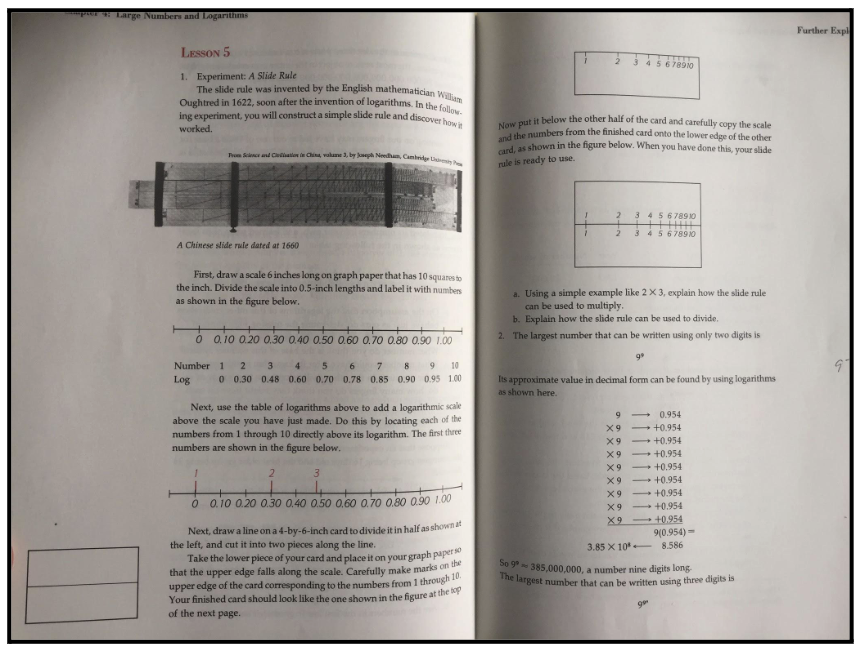
\includegraphics[width = 0.5\textwidth]{./Images/Jacobs No. 6.png}
        % \end{center}
    \end{statement}

    \begin{Highlight}[Solution]
        \begin{enumerate}[label=(\alph*)]
            \item To carry out the multiplication of $2 \times 3$ we move the $2$ on the sliding scale (depicted in \textcolor{red}{red}) to the $1$ on the fixed scale (depicted in \textcolor{yellow}{yellow}).
            We then move to the $3$ on the fixed scale and read the number that is aligned on the sliding scale, which is $6$. This can be seen in the image below.
            \begin{center}
                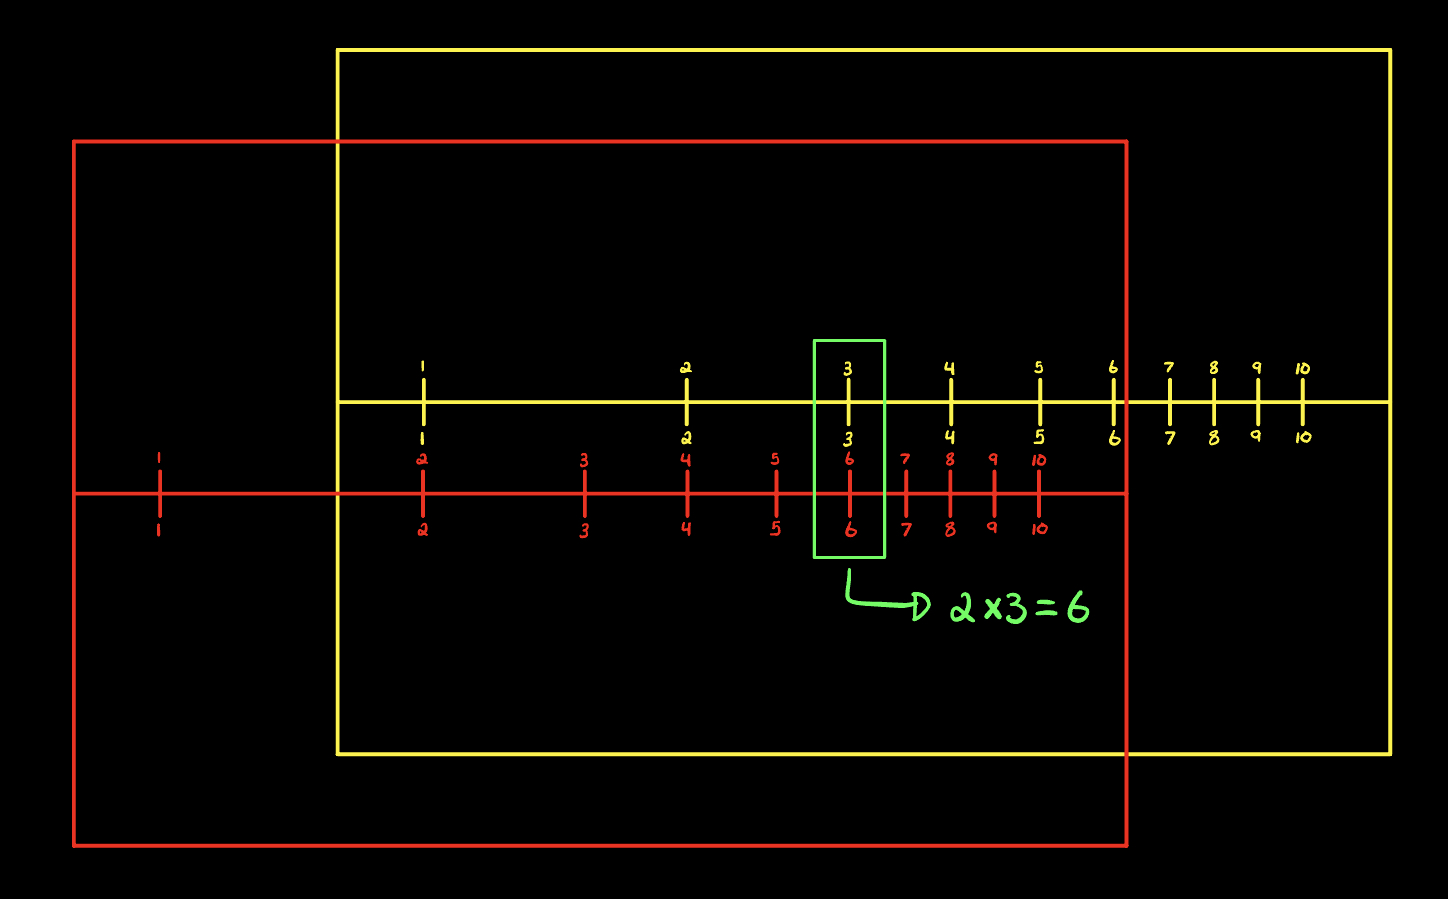
\includegraphics[width = 0.5\textwidth]{./Images/Slide Rule Multiplication.png}
            \end{center}
            \item To perform division, one moves the first value of the expression on the sliding scale to that of the second value of the expression on the fixed scale. Once this has been completed, the answer
            to the expression is then read off the value on the sliding scale that is aligned with the $1$ on the fixed scale. In this example, we are performing $8 / 4$ which is of course 2. This can be seen below.
            \begin{center}
                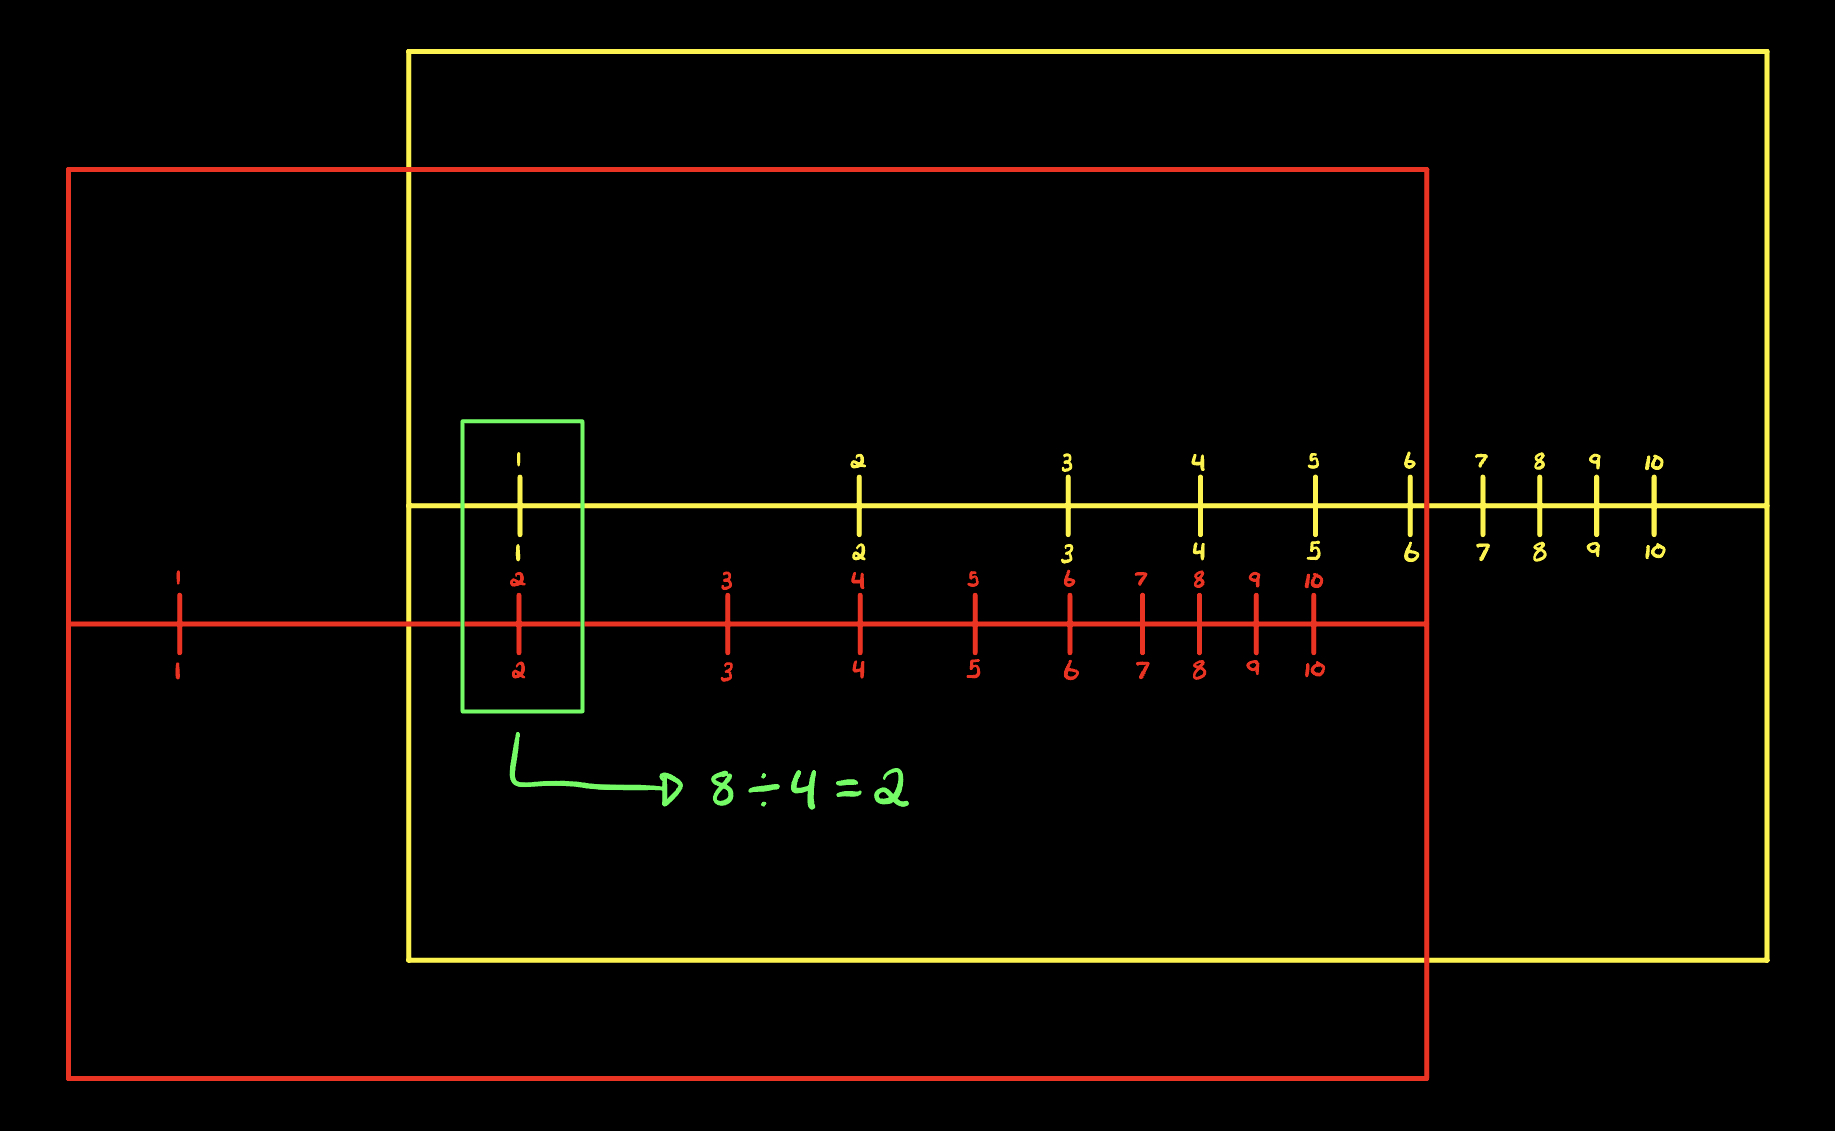
\includegraphics[width = 0.5\textwidth]{./Images/Slide Rule Division.png}
            \end{center}
        \end{enumerate}
    \end{Highlight}
\end{problem}

% Problem 6 Summary
\begin{summary}{Problem 6 Summary}
    \begin{statement}{Procedure}
        \begin{enumerate}[label = (\alph*)]
            \item To perform multiplication, line the second value of the expression on the sliding scale to that of the 1 on the fixed scale and read off the value of the sliding scale that is aligned with the second value
            of the expression on the fixed scale
            \item To perform division, line the first value of the expression on the sliding scale with that of the second value of the expression on the fixed scale and read off the value that is aligned with the 1 on the fixed
            scale
        \end{enumerate}
    \end{statement}
    \begin{statement}{Key Concepts}
        \begin{itemize}
            \item This problem utilizes how we can compute values with the use of a sliding scale
        \end{itemize}
    \end{statement}
    \begin{statement}{Variations}
        \begin{itemize}
            \item We could be asked to calculate different values on the sliding scale
            \begin{itemize}
                \item We would then use the same procedure with how to calculate the values on a sliding scale
            \end{itemize}
        \end{itemize}
    \end{statement}
\end{summary}

% Problem 7
\begin{problem}{Problem 7}
    \begin{statement}{Problem Statement}
        Do \#20/21 from Rosen p. 244 by hand and check your answers in the back or with a calculator.
    \end{statement}

    For these problems, I will be symbolizing \textbf{mod} with \%.

    \begin{Highlight}[Solution \#20]
        \begin{enumerate}[label = (\alph*)]
            \item $-17 \% 2 = 2 - (17 \% 2) = 2 - 1 = 1.$
            \item $144 \% 7 = 4.$
            \item $-101 \% 13 = 13 - (101 \% 13) = 13 - 10 = 3$
            \item $199 \% 19 = 9.$
        \end{enumerate}
    \end{Highlight}

    \begin{Highlight}[Solution \#21]
        \begin{enumerate}[label = (\alph*)]
            \item $13 \% 3 = 1.$
            \item $-97 \% 11 = 11 - (97 \% 11) = 11 - 9 = 2.$
            \item $155 \% 19 = 3.$
            \item $-221 \% 23 = 23 - (221 \% 23) = 23 - 14 - 9.$
        \end{enumerate}
    \end{Highlight}
\end{problem}

% Problem 7 Summary
\begin{summary}{Problem 7 Summary}
    \begin{statement}{Procedure}
        \begin{enumerate}[start = 20]
            \item Problem 20
            \begin{itemize}
                \item Use the rules of modulo to calculate the values
            \end{itemize}
            \item Problem 21
            \begin{itemize}
                \item Use the rules of modulo to calculate the values
            \end{itemize}
        \end{enumerate}
    \end{statement}
    \begin{statement}{Key Concepts}
        \begin{itemize}
            \item \textbf{Modulo Operation:} The modulo operation (denoted as $\%$) calculates the remainder when one number is divided by another. It is used to find the remainder of integer division
            \item \textbf{Calculation Process:} To find the result of a modulo operation, the following steps are typically followed:
            \begin{enumerate}
                \item The modulo operation is performed, e.g., $x \% y$, where $x$ and $y$ are numbers
                \item If the result is negative, it is adjusted to ensure it falls within the expected range, e.g ($-x \% y = y - (x \% y)$)
            \end{enumerate}
            \item \textbf{Generalization:} The concept of the modulo operation can be applied to any numbers $x$ and $y$. The key is to perform the division and adjust the result if necessary to obtain 
            a non-negative remainder
        \end{itemize}
    \end{statement}
    \begin{statement}{Variations}
        \begin{itemize}
            \item We could be asked to find the modulo of different numbers
            \begin{itemize}
                \item In this case we would use the same rules but with different numbers
            \end{itemize}
        \end{itemize}
    \end{statement}
\end{summary}

% Problem 8
\begin{problem}{Problem 8}
    \begin{statement}{Problem Statement}
        Do as many or \#30 - 33 p. 245 as needed (if you want to include your work in the MW add it at the end)  - these use the multiplication and adding rules on page 242. Use this shortcut. Then pick ONE 
        SINGLE ( for example 30 (b) or 33 (a) ) and on this page do the calculations 2 ways, one way doing each part (long way) and another by using the shortcuts from page 242. Hopefully you get the same 
        answers!
    \end{statement}

    For these problems, I will be symbolizing \textbf{mod} with \%.

    \begin{Highlight}[Solution - \#30]
        \noindent \textbf{Question:} Find each of these values. \vspace*{1em}

        \textbf{Shortcut Method:}
        \begin{enumerate}[label=(\alph*)]
            \item $(177 \% 31 + 270 \% 31) \% 31 = ((177 \% 31) \% 31 + (270 \% 31) \% 31) \% 31 = (22 \% 31 + 22 \% 31) \% 31 = 44 \% 31 = 13.$
            \item $(177 \% 31 \cdot 270 \% 31) \% 31 = ((177 \% 31)(270 \% 31)) \% 31 = ((22)(22)) \% 31 = 484 \% 31 = 19.$
        \end{enumerate}

        \textbf{Long Method:}
        \begin{enumerate}[label=(\alph*)]
            \item $(177 \% 31 + 270 \% 31) \% 31 = (22 + 22) \% 31 = 13.$
            \item $(177 \% 31 \cdot 270 \% 31) \% 31 = (22 \cdot 22) \% 31 = 19.$
        \end{enumerate}
    \end{Highlight}

    \begin{Highlight}[Solution - \#31]
        \noindent \textbf{Question:} Find each of these values.
        
        \begin{enumerate}[label=(\alph*)]
            \item $(-133 \% 23 + 261 \% 23) \% 23 = ((23 - (133 \% 23)) + 8) \% 23 = ((23 - 18) + 8) \% 23 = 13 \% 23 = 13.$
            \item $(457 \% 23 \cdot 182 \% 23) \% 23 = (20 \cdot 21) \% 23 = 420 \% 23 = 6.$
        \end{enumerate}
    \end{Highlight}

    \begin{Highlight}[Solution - \#32]
        \noindent \textbf{Question:} Find each of these values.

        \begin{enumerate}[label=(\alph*)]
            \item $(19^{2} \% 41) \% 9 = (361 \% 41) \% 9 = 33 \% 9 = 6.$
            \item $(32^{3} \% 13)^{2} \% 11 = (32768 \% 13)^{2} \& 11 = 8^{2} \% 11 = 64 \% 11 = 9.$
            \item $(7^{3} \% 23)^{2} \% 31 = (343 \% 23)^{2} \% 31 = (21)^{2} \% 31 = 441 \% 31 = 7.$
            \item $(21^{2} \% 15)^{3} \% 22 = (441 \% 15)^{3} \% 22 = 6^{3} \% 22 = 216 \% 22 = 18.$
        \end{enumerate}
    \end{Highlight}

    \begin{Highlight}[Solution - \#33]
        \noindent \textbf{Question:} Find each of these values.

        \begin{enumerate}[label=(\alph*)]
            \item $(99^{2} \% 32)^{3} \% 15 = (9801 \% 32)^{3} \% 15 = 9^{3} \% 15 = 729 \% 15 = 9.$
            \item $(3^{4} \% 17)^{2} \% 11 = (81 \% 17)^{2} \% 11 = 13^{2} \% 11 = 169 \% 11 = 4.$
            \item $(19^{3} \% 23)^{2} \% 31 = (6859 \% 23)^{2} \% 31 = 5^{2} \% 31 = 25 \% 31 = 25.$
            \item $(89^{3} \% 79)^{4} \% 26 = (704969 \% 79)^{4} \% 26 = 52^{4} \% 26 = 7311616 \% 26 = 0.$
        \end{enumerate}
    \end{Highlight}
\end{problem}

% Problem 8 Summary
\begin{summary}{Problem 8 Summary}
    \begin{statement}{Procedure}
        \begin{enumerate}[start = 30]
            \item Problem 30
            \begin{itemize}
                \item Use the rules of modulo to calculate the values
            \end{itemize}
            \item Problem 31
            \begin{itemize}
                \item Use the rules of modulo to calculate the values
            \end{itemize}
            \item Problem 32
            \begin{itemize}
                \item Use the rules of modulo to calculate the values
            \end{itemize}
            \item Problem 33
            \begin{itemize}
                \item Use the rules of modulo to calculate the values
            \end{itemize}
        \end{enumerate}
    \end{statement}
    \begin{statement}{Key Concepts}
        \begin{itemize}
            \item \textbf{Modulo Operation:} The modulo operation (denoted as $\%$) calculates the remainder when one number is divided by another. It is used to find the remainder of integer division
            \item \textbf{Calculation Process:} To find the result of a modulo operation, the following steps are typically followed:
            \begin{enumerate}
                \item The modulo operation is performed, e.g., $x \% y$, where $x$ and $y$ are numbers
                \item If the result is negative, it is adjusted to ensure it falls within the expected range, e.g ($-x \% y = y - (x \% y)$)
            \end{enumerate}
            \item \textbf{Generalization:} The concept of the modulo operation can be applied to any numbers $x$ and $y$. The key is to perform the division and adjust the result if necessary to obtain 
            a non-negative remainder
        \end{itemize}
    \end{statement}
    \begin{statement}{Variations}
        \begin{itemize}
            \item We could be asked to find the modulo of different numbers
            \begin{itemize}
                \item In this case we would use the same rules but with different numbers
            \end{itemize}
        \end{itemize}
    \end{statement}
\end{summary}

% Problem 9
\begin{problem}{Problem 9}
    \begin{statement}{Problem Statement}
        On the following page(s) explore the following with screenshots and explanations:

        \begin{itemize}
            \item Open up \href{https://www.desmos.com/}{Desmos.com}.
            \item Graph, imagine these are functions that show runtime ($y$) as a function of inputs ($x$)
            \begin{itemize}
                \item $f(x) = x$
                \item $g(x) = 1000 \log{x}$
            \end{itemize}
            \begin{enumerate}[label=(\alph*)]
                \item From looking at how these two graphs grow, as x gets larger and larger, which function seems to be showing a longer runtime?
                \item Is there a place on the graph where $g(x) = 1000 \log{(x)}$ is showing a longer runtime than $f(x) = x$?
                \item Does which function is `better' change as x gets big?
                \item Where on the x-axis does this happen?
                \item Where does it become clear that one of these is better (faster) runtime than the other?
            \end{enumerate}
            \item Experiment with other values of the log function:
            \begin{itemize}
                \item $p(x) = 10,000 \log{(x)}$
                \item $t(x) = 100,000 \log{(x)}$
            \end{itemize}
            \begin{enumerate}[label=(\alph*)]
                \setcounter{enumi}{5}
                \item Is $f(x)$ really `better' than these log functions as x gets large? Why or why not?
            \end{enumerate}
        \end{itemize}
    \end{statement}

    \begin{Highlight}[Solution]
        In the image on the left, $f(x)$ is the \textcolor{green}{green} line and $g(x)$ is the \textcolor{purple}{purple} line. For the added functions on the right, $p(x)$ is the \textcolor{red}{red} 
        line and $t(x)$ is the \textcolor{orange}{orange} line.
        \begin{center}
            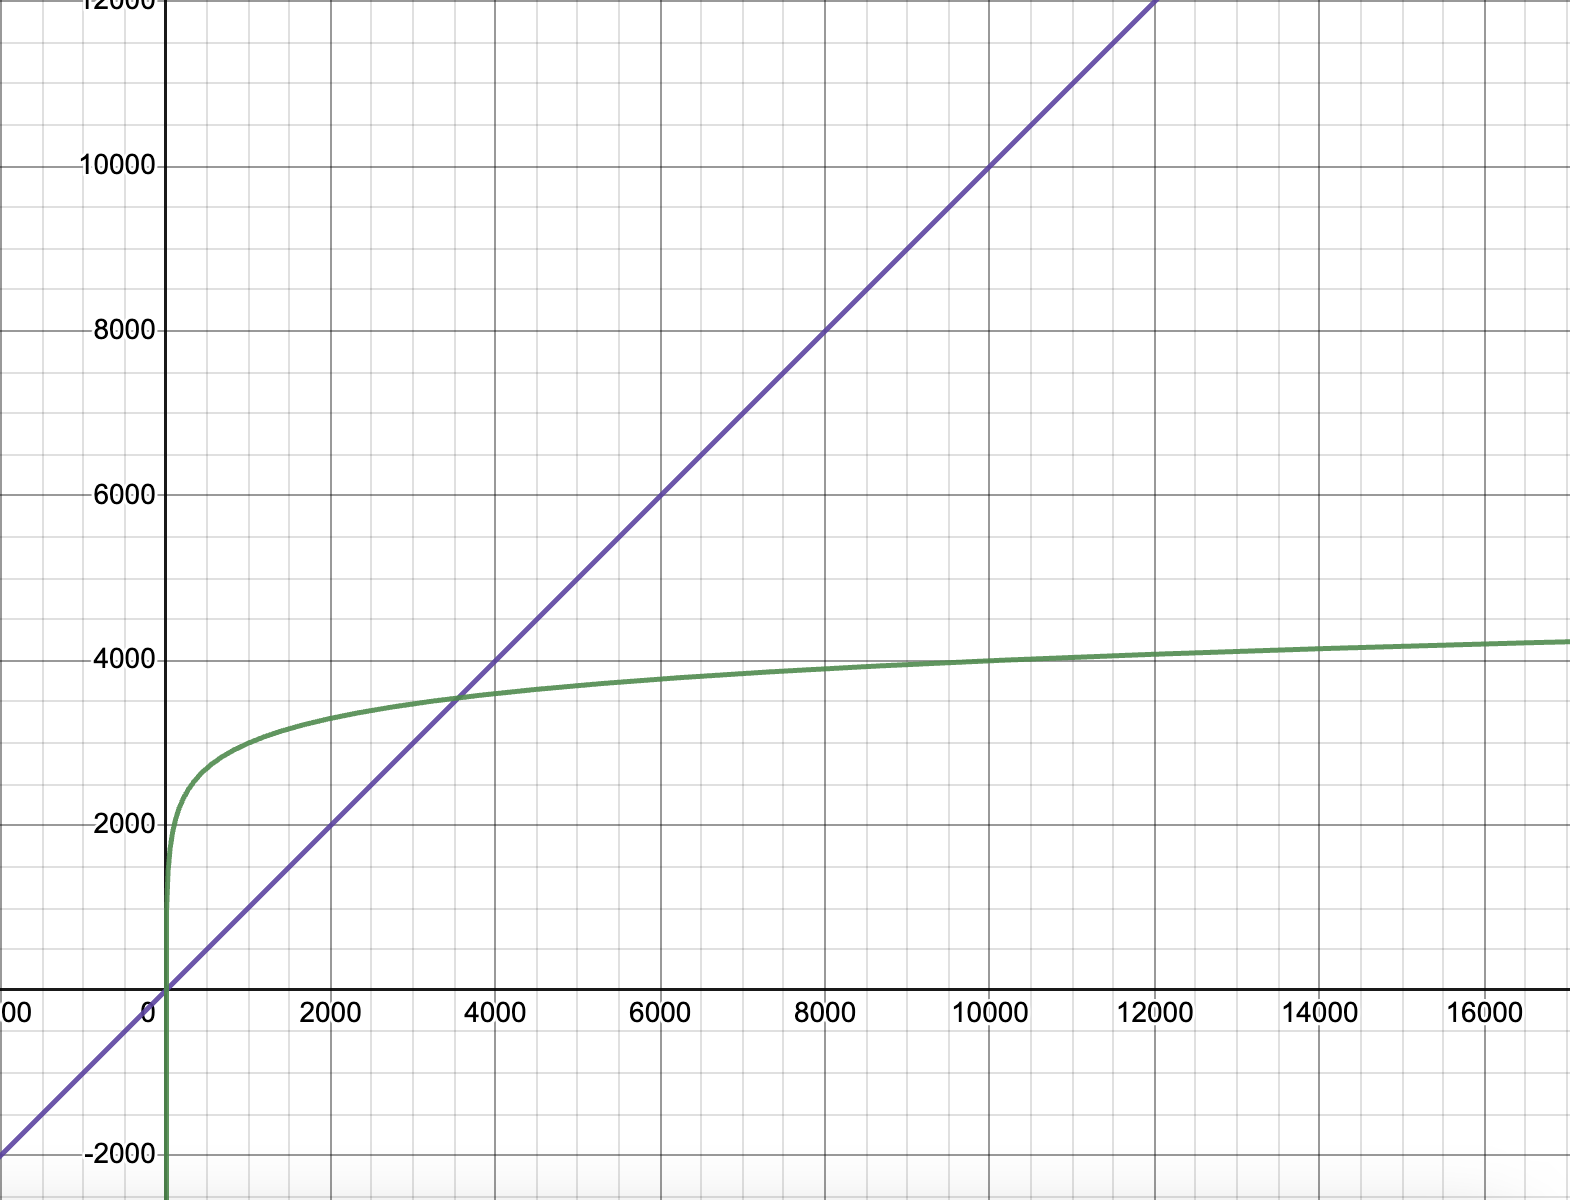
\includegraphics[width = 0.4\textwidth]{./Images/Desmos 1.png}
            \hspace{20pt}
            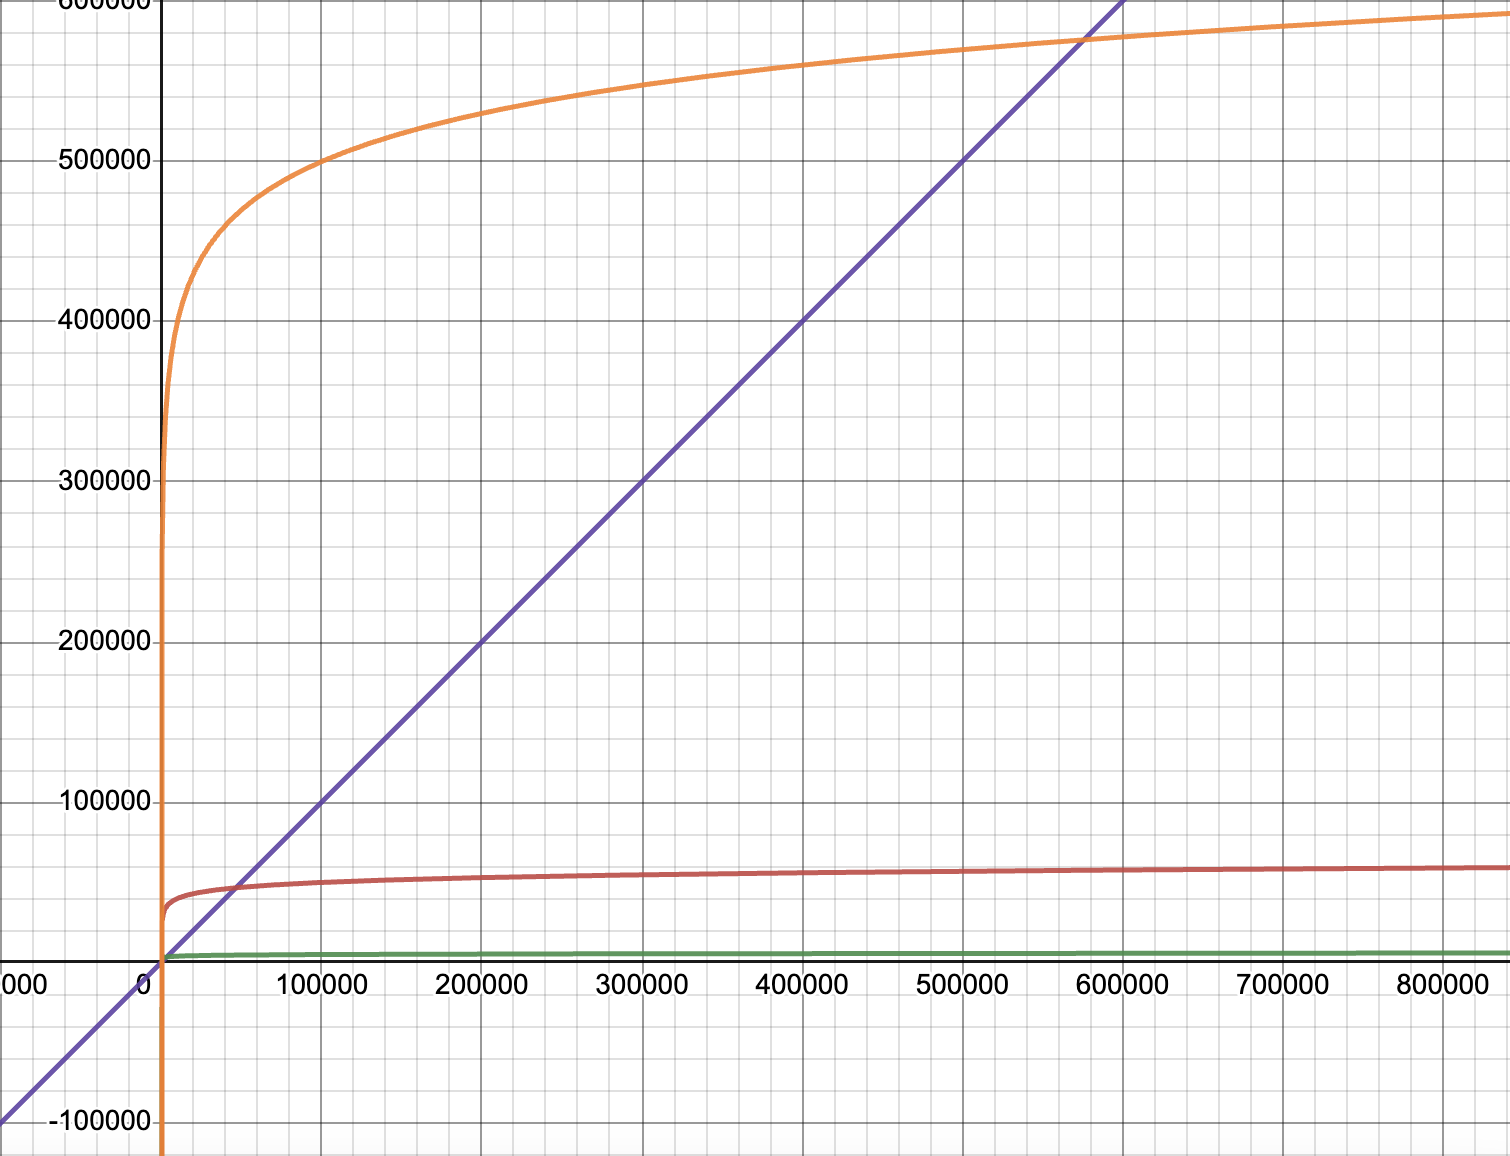
\includegraphics[width = 0.4\textwidth]{./Images/Desmos 2.png}
        \end{center}
        
        \begin{enumerate}[label=(\alph*)]
            \item As $x$ grows, $f(x)$ shows to have a longer runtime. This is because the $y$-axis represents the runtime and the $x$-axis represents the number of operations.
            \item Yes, up to the point $x \approx 3550$.
            \item As $x$ grows, it is easy to see that $g(x)$ is better for more operations.
            \item $g(x)$ is shown to be more efficient for values of $x > 3550$.
            \item Zoomed out on the graph, it is pretty obvious that $g(x)$ is more efficient than $f(x)$ for values of $x \geq 4000$.
            \item As $x$ gets large, $f(x)$ is not better. As the domain of the function grows, logarithmic functions tend to `level' out at a specific range value. Whereas the linear function $f(x)$ does not
            and it continues to grow linearly with an increasing $x$.
        \end{enumerate}
    \end{Highlight}
\end{problem}

% Problem 9 Summary
\begin{summary}{Problem 9 Summary}
    \begin{statement}{Procedure}
        \begin{itemize}
            \item Parts (a)-(f): Use Desmos and answer the prompts
        \end{itemize}
    \end{statement}
    \begin{statement}{Key Concepts}
        \begin{itemize}
            \item This problem encapsulates runtime efficiency for different $\mathcal{O}(n)$ types
        \end{itemize}
    \end{statement}
    \begin{statement}{Variations}
        \begin{itemize}
            \item We could be asked to look at different runtimes
            \begin{itemize}
                \item In this case we would use the same logic with different runtimes
            \end{itemize}
        \end{itemize}
    \end{statement}
\end{summary}